\documentclass[a4paper,11pt]{article}
\usepackage[utf8]{inputenc}
\usepackage[brazilian]{babel}
\usepackage{geometry}
\geometry{margin=0.7in, top=0.9in, bottom=0.8in}
\usepackage{xcolor}
\usepackage{paracol}
\usepackage{titlesec}
\usepackage{enumitem}
\usepackage{fontawesome5}
\usepackage[hidelinks]{hyperref}
\usepackage{lmodern}
\usepackage{graphicx}

\definecolor{primary}{RGB}{13,71,161}
\definecolor{accent}{RGB}{0,150,136}
\definecolor{graytxt}{RGB}{60,60,60}

\hypersetup{
    colorlinks=true,
    linkcolor=primary,
    urlcolor=primary
}

\setcolumnwidth{0.34\textwidth,0.62\textwidth}
\setlist[itemize]{noitemsep, leftmargin=*, label=\textbullet}

\titleformat{\section}
  {\large\bfseries\color{primary}}
  {}{0em}{\MakeUppercase}
  [\color{accent}\titlerule]

\titleformat{\subsection}
  {\normalsize\bfseries\color{accent}}
  {}{0em}{}

\newcommand{\sectionleft}[1]{\subsection*{#1}}
\newcommand{\sectionright}[1]{\section*{#1}}

\setlength{\parindent}{0pt}

\begin{document}

\begin{center}
    {\LARGE\bfseries\color{primary} Fernando Anselmo}\\[2mm]
    {\large\color{graytxt} Líder Técnico Full Stack | Arquitecto de Soluciones | Profesor}\\[4mm]
    \begin{tabular}{@{}l@{}}
        \faIcon{map-marker} Brasília - DF, Brasil \quad
        \faIcon{envelope} \href{mailto:fernando.anselmo74@gmail.com}{fernando.anselmo74@gmail.com} \\
        \faIcon{phone} (61) 99874-0763 \quad
        \faIcon{linkedin} \href{https://www.linkedin.com/in/fernando-anselmo-bb423623/}{LinkedIn} \quad
        \faIcon{github} \href{https://github.com/fernandoans}{GitHub}
    \end{tabular}
\end{center}
\vspace{2pt}

\section*{Resumen Profesional}
Líder técnico estratégico con más de 35 años de experiencia en proyectos críticos de alto rendimiento. Especializado en transformar complejidad técnica en soluciones claras y eficientes con resultados concretos y sostenibles. Autor de 18 libros, conferencista y profesor. Especialista en modernización de legados, CI/CD, integraciones corporativas y arquitecturas Hexagonal y de Microservicios.
\vspace{2pt}

\begin{paracol}{2}

\sectionleft{Competencias Principales}
\begin{itemize}
    \item Java, Spring Boot
    \item Quarkus
    \item J2EE, Struts
    \item Angular 17/21, TypeScript
    \item Node.js, React, React.Native
    \item Docker, Jenkins, Azure DevOps
    \item GitLab CI
    \item PostgreSQL, Oracle, SQL Server
    \item MongoDB, Cassandra, Neo4J
    \item AWS, Oracle Cloud
    \item Arquitectura Hexagonal
    \item Microservicios, DevSecOps
\end{itemize}

\vspace{4pt}
\sectionleft{Certificaciones}
\begin{itemize}
    \item \textbf{Java Champion – Oracle}
    \item Certified AI Foundations Associate
    \item Certified Programmer Java
    \item Certified Web Developer Java
    \item SCRUM Foundation
\end{itemize}

\vspace{4pt}
\sectionleft{Idiomas}
\begin{itemize}
    \item Inglés – habla, lectura y escritura
    \item Español – habla, lectura y escritura
\end{itemize}

\switchcolumn

\sectionright{Experiencia Profesional}

\textbf{Desarrollador FullStack Senior – First Decision} \\
\textit{Ministerio de Transportes / Mauá FalaBr}
\hfill ene/2025 – presente
\begin{itemize}
    \item Angular 17/21 + Java Spring Boot Hexagonal Ports and Adapters
    \item Estructuración de entornos con segmentación de red y seguridad
    \item Integraciones PostgreSQL, SQL Server, Oracle y microservicios
    \item Apoyo arquitectónico con IA en Node.js/TypeScript
\end{itemize}

\textbf{Desarrollador FullStack Senior – Qintess} \\
\textit{Ministerio de Transportes}
\hfill ago/2024 – ene/2025
\begin{itemize}
    \item Java/Angular con arquitectura Hexagonal
    \item Gobierno de Git, APIs REST
\end{itemize}

\textbf{Desarrollador Backend Java – SEA Tecnologia} \\
\textit{PesqBrasil / Portal SESC}
\hfill nov/2024 – mar/2025
\begin{itemize}
    \item Liferay Java, DevSecOps, observabilidad
    \item Pipelines CI/CD, planeación de capacidad, alta disponibilidad
\end{itemize}

\textbf{Analista de Sistemas IV – CNI/SESI} \hfill nov/2021 – oct/2024
\begin{itemize}
    \item Refactorización Java heredado, APIs, Jasper Reports, AD
    \item OutSystems, Power Apps/Power Automate
    \item Kubernetes, GitLab CI/Jenkins, DevSecOps
\end{itemize}

\textbf{Arquitecto de Soluciones – Bancorbrás} \hfill feb/2021 – nov/2021
\begin{itemize}
    \item Spring Boot, Quarkus/GraalVM, CI Docker/Jenkins/SonarQube
    \item Modernización de Stored Procedures, integración Protheus/AD
\end{itemize}

\textbf{Desarrollador Backend – Mirante Tecnologia} \hfill oct/2019 – feb/2021
\begin{itemize}
    \item Microservicios Spring Boot, Jenkins/Docker
    \item Oracle Cloud, TDD, integraciones corporativas
\end{itemize}

\textbf{Trabajos anteriores} \hfill 1987 – oct/2019
\begin{itemize}
	\item Consulte mi LinkedIn para ver la relación completa
	\item \href{https://www.linkedin.com/in/fernando-anselmo-bb423623/}{Acceder a LinkedIn}
\end{itemize}

\end{paracol}

\section*{Experiencia Docente}
\textbf{Profesor de Informática -- UDF - Grupo Cruzeiro do Sul} \hfill feb/2023 – presente\\
Grado en Tecnología de la Información – Algoritmos, POO, Móvil, Web, Backend y Móvil.

\textbf{Profesor de Ciencia de Datos -- IESB} \hfill ago/2018 – presente\\
Grado/Posgrado – Python, Hadoop, Java, Móvil, Robótica y Automatización.

\vspace{4pt}

\section*{Formación Académica}
\begin{itemize}
	\item Posgrado en Docencia en Sistemas de Información - Faculdade Iguaçu - En curso
	\item Posgrado en Arquitectura de Software - Faculdade Iguaçu - En curso
	\item MBA en Gestión de la Información - Faculdade Iguaçu - En curso
	\item MBA en Tecnología para Negocios: Data Science y Big Data - Faculdade Iguaçu - En curso
	\item Posgrado en competencia en tecnologías digitales para educación emprendedora - Secretaria de Educación GDF / SEBRAE - En curso
	\item Posgrado en Estadística Aplicada - Faculdade Anhanguera - 2020
	\item Técnico en Juegos Digitales - IFB - 2019
	\item Posgrado en Gestión Empresarial Avanzada - Faculdade JK - 2016
	\item Licenciatura en Gestión de Tecnología de la Información - FacSenac - 2011
	\item Especialización en Programación - Faculdades Integradas da Católica - 1996
\end{itemize}

\section*{Mapa de Competencias}
\begin{center}
    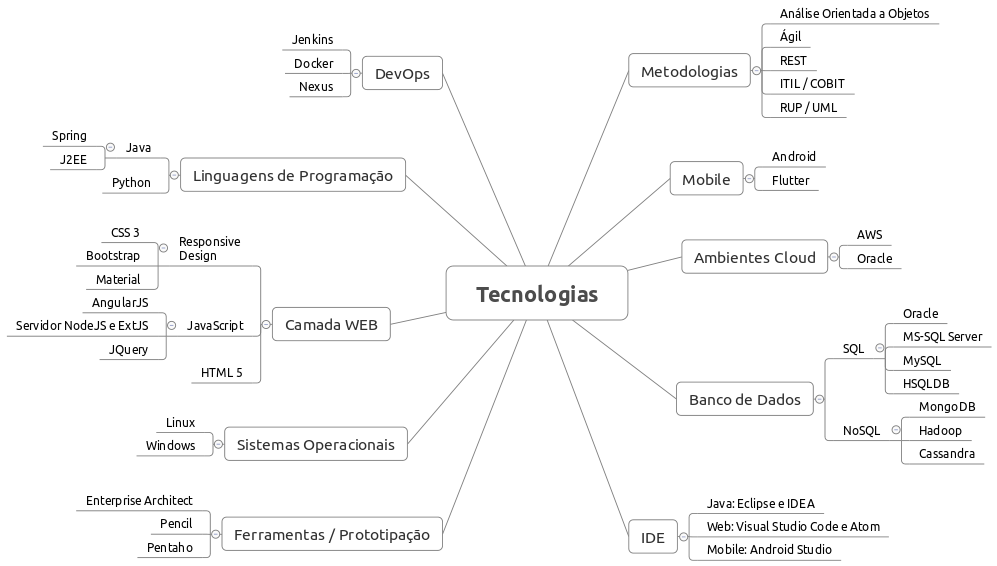
\includegraphics[width=0.95\textwidth]{imagens/tecnologias.png}
\end{center}

\end{document}
